\chapter{Les Interfaces}
Pour une consultation plus précise des interfaces, veuillez vous référer à notre projet sur Figma.
\url{https://www.figma.com/file/qPQb27LuO5XC7c0dZNxZG4/Rissala-Project-UI?type=design&node-id=0-1&mode=design&t=kXxYedrESPdWnNO0-0}
section{les privilèges de chaque acteur}
\subsubsection{Admin}
L'administrateur a le privilège de gérer l'intégralité de la plateforme.



\subsubsection{Le créateur de contenu}
En tant que créateur de contenu, il est nécessaire de se connecter pour accéder à son profil et créer des newsletters. Par ailleurs, vous avez la possibilité de consulter les newsletters créées par d'autres utilisateurs, comme illustré dans le diagramme du cas d'utilisation. 
\subsubsection{guest}
En tant qu'invité, vous avez la possibilité de rechercher des newsletters, de vous y abonner, de consulter les newsletters ainsi que les créateurs de contenu.
\section{interfaces}
\clearpage
\begin{figure}[htbp]
    \centering
    \begin{minipage}[b]{0.7\textwidth}
        \centering
        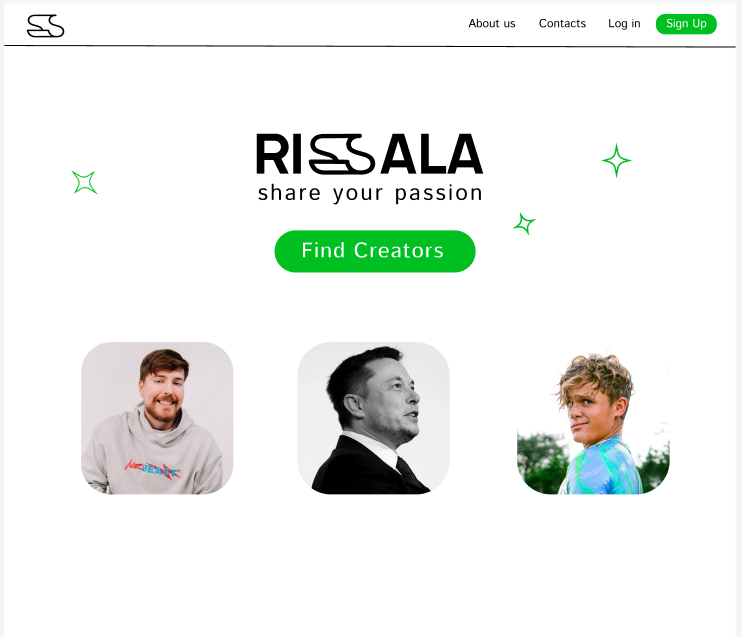
\includegraphics[width=\textwidth]{interfaces/index.png}
        \caption{Index}
        \label{fig:index}
    \end{minipage}
    \hfill
    \begin{minipage}[b]{0.7\textwidth}
        \centering
        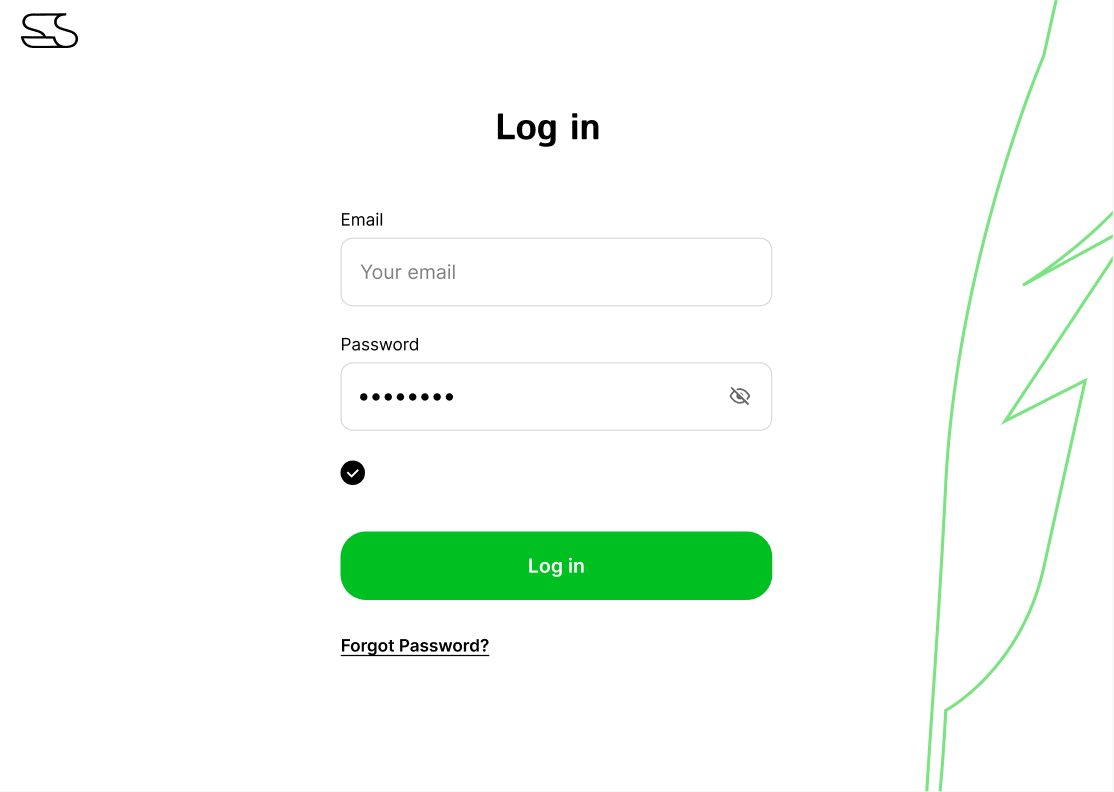
\includegraphics[width=\textwidth]{interfaces/log in.png}
        \caption{Log in}
        \label{fig:connexion}
    \end{minipage}
\end{figure}
\begin{figure}
    \centering
    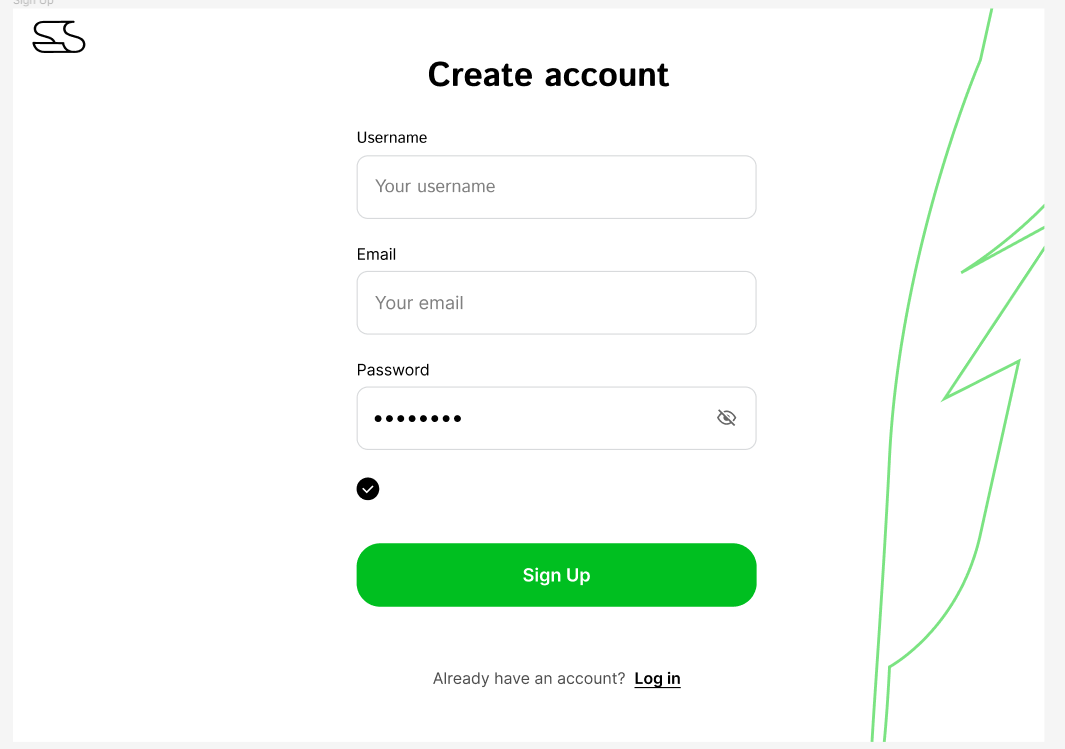
\includegraphics[width=0.7\textwidth,height=1\textheight,keepaspectratio]{interfaces/sign up.png}
    \caption{Sign in}
    \label{fig:diagramme}
\end{figure}
\begin{figure}
    \centering
    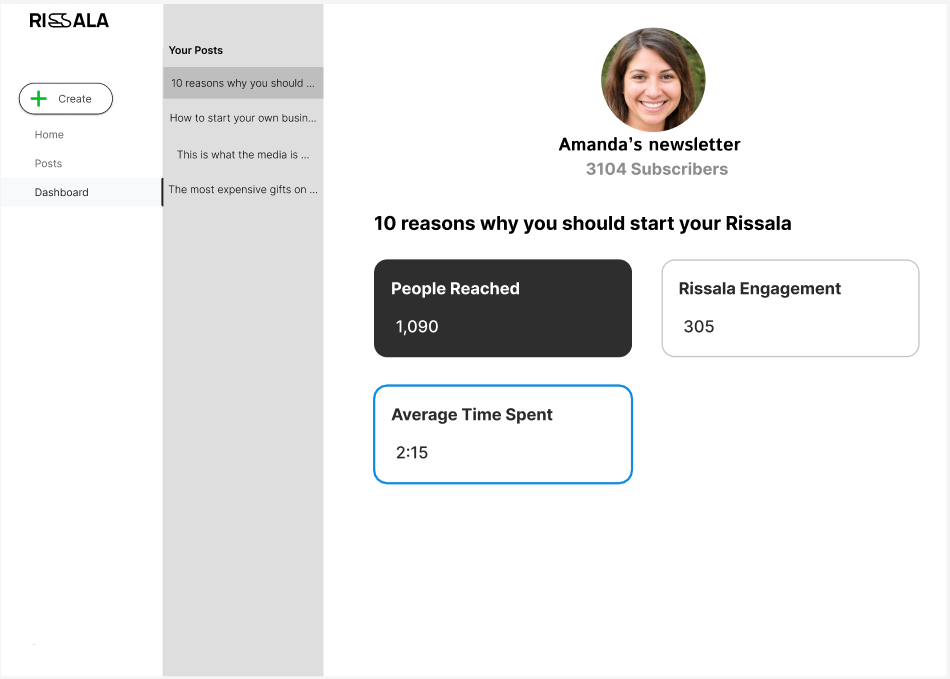
\includegraphics[width=0.7\textwidth,height=1\textheight,keepaspectratio]{interfaces/Dashboard.png}
    \caption{Dashboard}
    \label{fig:diagramme}
\end{figure}
\begin{figure}
    \centering
    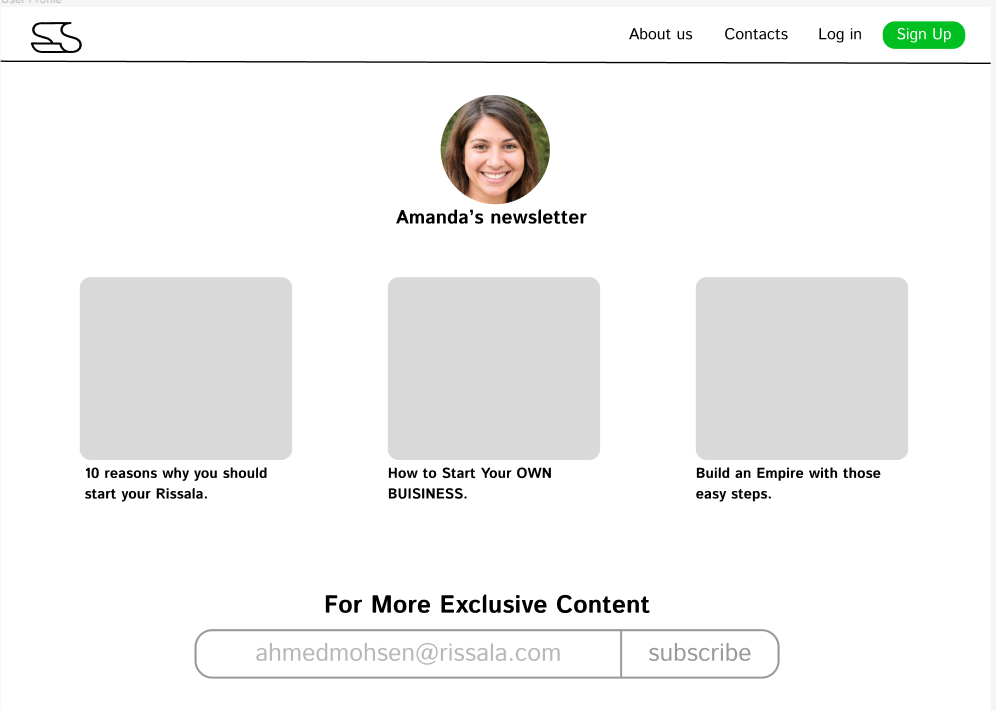
\includegraphics[width=0.7\textwidth,height=1\textheight,keepaspectratio]{interfaces/user profile.png}
    \caption{Profile}
    \label{fig:diagramme}
\end{figure}
\begin{figure}
    \centering
    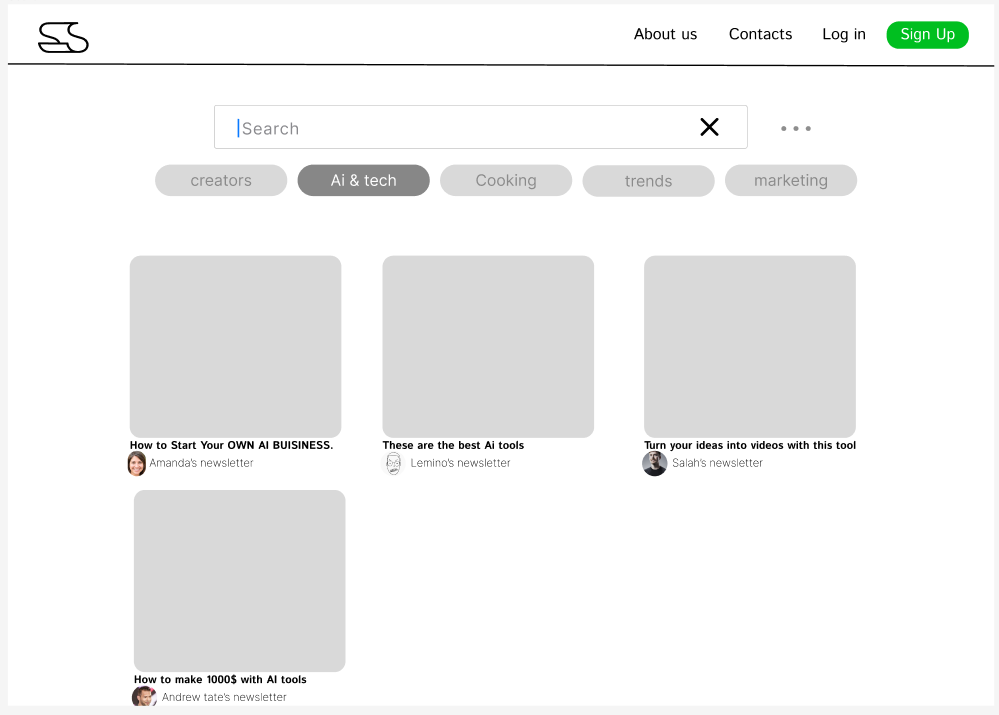
\includegraphics[width=0.7\textwidth,height=1\textheight,keepaspectratio]{interfaces/search.png}
    \caption{Search}
    \label{fig:diagramme}
\end{figure}
\begin{figure}
    \centering
    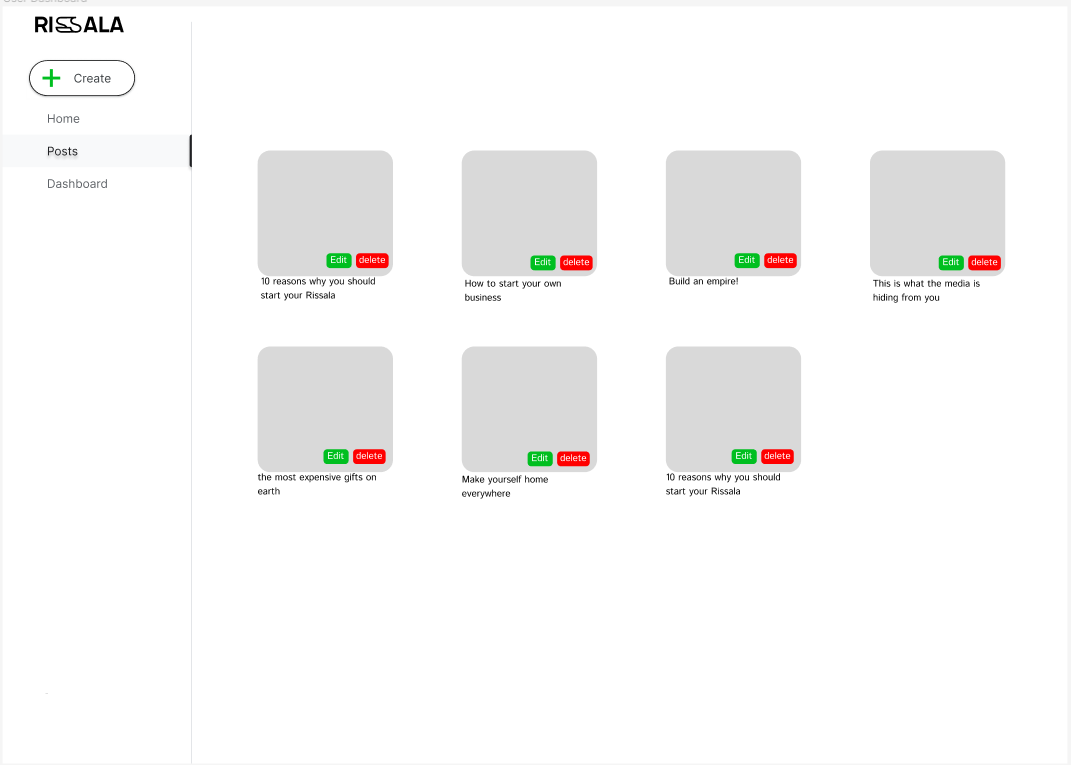
\includegraphics[width=0.7\textwidth,height=1\textheight,keepaspectratio]{interfaces/posts.png}
    \caption{Postes}
    \label{fig:diagramme}
\end{figure}